\documentclass{seminar}
\usepackage[french]{babel}
\usepackage{amsmath}
\usepackage{graphicx}
\usepackage{panther-slides}
\usepackage{url}


\pantherbeg
  \vspace*{26pt}
  \begin{flushright}
  \begin{bf}\begin{it}
      
      \begin{LARGE}
	\realbig
	 Different ways of annotating and \\proving
	 a quicksort with Jack\\[10pt]
      \end{LARGE}
  \end{it} \end{bf}
  \norm
  Julien Charles\\
%Benjamin Gr\a'egoire\\
\vfill
\begin{minipage}{5cm}\small
%\begin{flushright}
%Benjamin Gr\a'egoire
%\end{flushright}
%\begin{tabbing}
% \=Benjamin Gr\a'egoire\\ \>Benjamin Gr\a'egoire
%\end{tabbing} 
\end{minipage}\\
  \small
  \begin{tabular}{p{0.7\linewidth}r}
  
\epsfig{file=everest_logo.ps, height=18pt} & Thursday, february the 16th 2006\\
  \end{tabular}

  \end{flushright}
 %
\epsfig{file=logo.eps, height=18pt}
  

\nextslide{Introduction}

\blist
\small 
\item Goal: verify  a {\purple quicksort} written in Java 
  annotated with {\purple JML} with Jack
\item \ {\purple Static verification} of this program: \\
\rarrow done in an interactive way with Coq.
\item Motivation: need for some simple examples in Jack
  \blist 
    \item Already done in ESC/Java2
    \item Already done in Krakatoa\\
    \rarrow Now doing it in {\purple Jack}
  \elist 
\item It is still a work in progress \\(the proof not using the predicates is
finished,  not the other)
\elist
\nextslide{General Plan}
\begin{enumerate}
\item Basics
\item Annotating in a normal way
\item Using purity  
\item Using ghost and model variables
\end{enumerate}


\nextslide{Basics}
\begin{enumerate}
\item{The Java Modelling Language (JML)}
\item{Jack}
\item{Coq}
\end{enumerate}

\nextslide{JML}\small
The {\purple Java Modelling Language} (JML)
is used to annotate the Java programs we want to verify with 
Jack.\\
%Jack use a {\purple weakest precondition calculus} to generate
%the proof obligations.\\
In JML you can express loop invariants, assertions method's
pre and post conditions.\\
JML has a really large syntax so every tool (except maybe JMLrac)
implements only a {\purple portion} of its syntax.
\nextslide{JML constructions used (1)}
\small
\blist
\item Expressions used in annotations are special {\purple boolean expressions}:
\blist
  \item $\backslash$forall
  \item $\backslash$exists
  \item $\backslash$old
  \item methods if they are pure
\elist
\item Methods:
  \blist 
  \item requires 
  \item ensures
  \item modifies
  \elist
\item Assertions with the {\purple assert} construct
\elist
\nextslide{JML constructions used (2)}
\small
\blist
\item Loop invariants, termination:
  \blist 
  \item loop\_invariant
  \item decreases
  \item \ {\purple loop\_modifies}
  \elist
\item ghost variables
  \blist
  \item ghost v;
  \item set v = value;
  \elist
\elist
\nextslide{Jack (1)}
\small
\blist
\item Programmed mainly by {\purple Lilian Burdy}
\item Uses a {\purple weakest precondition calculus} to generate proof obligations
\item The proof obligations are decomposed w.r.t. the different 
{\purple execution cases}
\elist
\begin{center}
\includegraphics[width= \linewidth]{jack.ps}
\end{center}
\nextslide{Jack (2)}
\small
\blist
\item At first single prover (B)
\item Multi-prover interface (Simplify, Coq, PVS)
\item Fully integrated in {\purple Eclipse} as a plugin, and use a 
{\purple plugin architecture} to include new provers
\item To prove the quicksort we used the {\purple Coq Output} from Jack
\item Coq plugin in can be both used to prove {\purple automatically and
interactively} the proof obligations generated by Jack
\elist

\nextslide{Coq}
\small
Coq is based on the {\purple calculus of inductive constructions}.\\
You can express: types, axioms, functions
variables, definitions, {\purple lemmas}...

Lemmas have to be proved.\\
To prove a lemma you have to build a {\purple proof term} out of the types, 
axioms, variables... \\
To build this proof term you use special commands 
called {\purple tactics} within a proof script.

{\purple Custom tactics} can be created composing more primitive ones.\\

It can easily express the logics for Jack.
\nextslide{Coq with Jack}
\small
The files generated by Jack in Coq can be separated into 3 categories:
\blist 
\item The {\purple prelude} containing the logic used :
\blist 
\item A static part (jack.arith.v jack.references.v jack.tactics.v)
\item A dynamic part generated for a specified class (myClass.classes.v 
myClass.subtypes.v myClass.v)

\elist
\item The {\purple proof obligation} (1 file)
\item A file containing some {\purple custom tactics} written by the user
\elist
To edit the files we use the {\purple CoqEditor} plugin, an integrated editor for Coq files in Eclipse.

\nextslide{Annotating in a normal way}
\begin{enumerate}
\item{The QuickSort algorithm}
\item{Kind of proof obligations}
\item{Annotations}
\item{A tactic: eassert}

\end{enumerate}

\nextslide{The QuickSort algorithm...}
\small
\begin{tabbing}
pri\=vate void sort(int lo, int hi) \{\+ \\
  int left, right, pivot;\\
  if(!(lo $<$ hi)) return;\\
  left = lo;\\
  right = hi;\\
  pivot = tab[hi];\\
  
  whi\=le(left $<$ right) \+\{\\
    while((left $<$ right) \&\& (tab[left] $<=$ pivot)) left++;\\
    while((left $<$ right) \&\& (tab[right] $>=$ pivot)) right--;\\
    if\=(left $<$ right)\+ \{\\
      swap(left, right);\-\\
    \}\-\\
  \}
\end{tabbing}
\nextslide{...in Java}
\small
\begin{tabbing}
\ \ \ \=swap(left, hi);\+\\
  if \=(left $>$ 0)\+\\
  sort(lo, left -1);\-\\
  
  if (left +1 $<$ tab.length)\+\\
  sort(left +1, hi);\- \-\\
\}
\end{tabbing}

\blist
\item Property wanted: it sorts the array
\item The permutation property is left out, we use just an {\purple injection} property
\elist
\nextslide{Kind of proof obligations}
\small
\blist
\item Around 230 proof obligations (POs)
\item 100 are solved automatically
\item Difficulties: 
\blist 
\item the {\purple loop termination} wasn't so trivial\\
\rarrow the use of {\purple ghost variables} was necessary
\item the proof can easily get {\purple messy}\\
\rarrow use of assertions
\elist
\elist
\nextslide{Annotations (1)}
\small
Specifications of the main method:
\begin{tabbing}
/*\=@ {\purple requ}\={\purple ires} (tab != null) \&\& (0 $<=$ lo) \&\& (lo $<$ tab.length) \&\&\+ \\
  @     \>(0 $<=$ hi) \&\& (hi $<$ tab.length);\\
    @ {\purple modifies} tab[lo .. hi];\\
    @ {\purple ensures} ($\backslash$forall int i, j; (lo $<=$ i) \&\& (i $<=$ hi) $==>$ (lo $<=$ j) \&\& (j $<=$ hi) \\
    @             \> $==>$ (i $<$ j) $==>$ tab[i] $<=$ tab[j]) \&\&\\
    @             \>($\backslash$forall int i\=; lo $<=$ i \&\& i $<=$ hi; ($\backslash$exists int j; lo $<=$ j \&\& j $<=$ hi \&\& \\
 @ \>\>$\backslash$old(tab[j]) == tab[i])); \\
    @*/\\
        private void sort(int lo, int hi)\\
\end{tabbing}
\nextslide{Annotations (2)}
\small
Annotations of the loop invariant:
\begin{tabbing}
/*\=@ {\purple loop\_modifies} left, right, tab[lo..(hi - 1)];\+\\
  @ {\purple loop\_}\={\purple invariant} \= (lo $<=$ left) \&\& (left $<=$ right) \&\& (right $<=$ hi) \&\& \\
  @    \>($\backslash$forall int m; (lo $<=$ m) \&\& (m $<$ left) $==>$ tab[m] $<=$ pivot) \\
  @    \>\&\& ($\backslash$forall int n; (right $<$ n) \&\& (n $<=$ hi) $==>$ pivot  $<=$ tab[n])\\
  @     \>\&\& tab[right] $>=$ pivot \&\&\\
  @     \> ($\backslash$forall int i; lo $<=$ i \&\& i $<=$ hi - 1; \\
@ \>\>($\backslash$exists int j; lo $<=$ j \&\& j $<=$ hi \&\& $\backslash$old(tab[j]) == tab[i]));\\
  @ {\purple decreases} (right - left);\\
  @*/
\end{tabbing}
\nextslide{A tactic: eassert (1)}
\small
Many of the goals in this proofs were with {\purple split inequalities}
\blist
\item The hypothesis were of the form:\\
H: $\forall$ v, A \rarrow B(v)... \rarrow a $<$ b\\
H': $\forall$ v, A' \rarrow B'(v)... \rarrow b $<$ c
\item the lemma to prove:\\
a $<$ c
\item
I had troubles {\purple directly} instanciating the hypothesis to have:\\
a $<$ b and b $<$ c.
\elist
\rarrow the tactic {\purple eassert}
\nextslide{eassert (2)}
\small
The tactic is like assert, but it permits {\purple holes} when
instanciating the hypothesis, and the  holes are turn 
{\purple into subgoals}.\\
For a goal like:\\
H: A \rarrow B \rarrow C\\
=========================\\
G


eassert(h := H \_ \_).\\
turns it into {\purple 3 goals}:
\blist
\item One in order to prove A
\item One in order to prove B
\item One still asking to prove G
but with an hypothesis added (h: C)
\elist

\section{Pure methods}
JML's pure methods are methods that can be used in specifications.
They cannot mutate already existing objects but they can allocate new objects.
Nonetheless, the pure keyword is not an alias for JML {\tt modifies $\backslash$nothing}, 
it implies also that the methods terminates, giving a result or throwing an 
exception.
For instance if a constructor only modifies the object that is being 
created and terminates properly
it can be considered as pure.
A mean to verify whether a method is pure or not according to JML
can be found in \cite{salcianu05}. 



In dynamic program verification pure methods are usually built from their source code. 
The method is first thought on the Java level, without side effects, and afterward
the user writes its specifications on the JML level; in order to be able
to use it in JML annotations.

In static program verification,  pure methods can be built directly
from their specifications, since most of the tools replace  pure method's calls 
 by the instanciation of the pure method's specifications.


\subsection{Jack's implementation}
In Jack the notion of purity used is as in JML a kind of observational purity \cite{naumann05}, 
but a constructor that
only modifies the fields of the newly created objects is not considered 
as pure.
In Jack's weakest precondition calculus the specifications are considered 
as lightweight: the method calls are replaced by their specifications 
inside the calculus.
The replacement with its specifications is done with the normal 
specifications in case the method terminated normally or with the 
exceptional specification if the pure method terminated on an exception.
 
For a method defined in a Java file: 
\btab
 /*\=@ requires tab != null;\+\\
  @  modifies $\backslash$nothing;\\
  @ ensures   $\backslash$result == (0 $\le$ i) \&\& (i $\le$ tab.length);\\
  @ exsures false;\\
  @*/\-\\
publi\=c static /*@ pure @*/  withinBounds(int[] tab, int i) \{\+\\
       return (0 $\le$ i) \&\& (i $\le$ tab.length);\-\\
\}
\etab

with this method call within the annotations: 
\btab
withinBounds(tab,i)
\etab

the method call will be directly replaced in the weakest precondition calculus by:
\btab
(tab $!=$ null) \rarrow \ (0 $\le$ i) \conj \ (i $\le$ tab.length)
\etab
Since the specification
of the method has an {\tt exsures false} clause, there is no exceptional case.
In a way, this method will be replaced by its specifications like for a macro.



\subsection{Specification macros}


When specifying a program with JML one of the main problem is the 
growth of the size of the annotations. 
The way static verification tools usually define the handling 
of pure methods, we can use them to do some specification macros.
The method calls will be replaced by their specifications when the 
annotations will be interpreted. It is useful to avoid the growth.

If we have for instance a property to tell an array is sorted we would 
prefer read the annotation:
\btab
is\_sorted(tab)
\etab
instead of:
\btab
 $\backslash$forall \=int i; 0 $\le$ i \&\& i $<$ tab.length;\+\\ 
 $\backslash$forall int j; \=0 $\le$ j \&\& j $<$ tab.length; \+\\(i $<$ j) ==$>$ tab[i] $\le$ tab[j];
\etab
This method makes the annotations clearer, but as annotations 
grows big, proof obligations grows big too. In order to ease the readability 
of the proof obligations, we would like to keep track of the pure method name
that was used as the macro in order to see what part of the specification we 
are proving. That's why we changed the pure method's substitution in Jack.

In Jack, we decided to have a couple Definition / hypothesis.
Now a functional definition is generated of the form:
\btab
mypurefun\_norm  Args Result := (requires Args) \rarrow \ (ensures Args Result)\\
mypurefun\_exc  Args Result := (requires Args) \rarrow \ (exsures Args Result)
\etab
where {\tt requires} is a predicate that is on the arguments of the pure function and 
which correspond to JML {\tt requires} clause the same for {\tt ensures} and {\tt exsures} 
which are predicates that correspond to JML's {\tt ensures} and {\tt exsures} clause respectively.
These functions are then called within the hypothesis at the places where they were used in the code. 

It is nearly what is done in Krakatoa\cite{MPMU-04-JLAP}, as
Krakatoa use a functional definition of the pure method if it can generate it
but otherwise use an axiomatisation of it like in ESC/Java\cite{COKK-04-ESCJ}.
The axiomatisation is done in 3 parts: the pure method is first declared as a variable, 
there is some hypothesis  using it and giving it its properties (which correspond to its
specifications), and then the variable
is used within the lemma which has to be proved (for more detailed comparison between 
the different technique see: \cite{COK-04-METH, DarvasMueller-05}).

This way of defining Definition/Hypothesis doesn't change anything for automatic 
proof of the proof obligations with prover like Simplify. 
%However, with Coq 
%it add an extra step to the proof which is to unfold the definition 
%within the hypothesis. Nevertheless,  
With Coq,
it facilitate the readability of the proof obligation for the user which 
is a critical point, notably when doing an interactive proof.

\subsection{Pure as Predicates}
Some of the properties we have to express are not so easy to deal with on the JML level. 
We want to be able to prove lemmas concerning pure methods, and also have 
relations over  variables without specifying any property on the relation. 

So we decided to be able to define pure methods directly within the language in which the proof 
obligations are generated or the JML annotations are interpreted. 
We added a new keyword to JML in order to allow it: the {\tt native} keyword. 
If a method is declared within a specification as native, the method will not be defined nor specified
 in JML at all, it will only be declared. Its specifications will be to the target prover or environment 
discretion.

Since the native methods are declared within the specifications they must be pure:
they must not have any side-effect, they can only
create new objects, they have to be terminating. But native is
more restrictive than pure: a native method must not throw any exception.


For instance we can have the property {\tt withinBounds} declared as native, inside the specification:
\btab
//@ public native static boolean withinBounds(int [] tab, int i); 
\etab
If interpreted with a dynamic program verification tool, it
can be defined with the Java method:
\btab
public \= static boolean withinBounds(int [] tab, int i) \{\+\\
    return (tab $!=$ null) \&\& (0 $\le$ i) \&\& (i $\le$ (tab.length));\-\\
\}
\etab
If interpreted with a static program verification tool,
it can be defined this way in Coq:
\btab
Def\=inition withinBounds := \+\\
fun \= (tab i) =>\+\\
       (and (not (tab = null)) (and (0 $\le$ i) (i $\le$ (arraylength tab))).
\etab
In Simplify it will be seen as an uninterpreted function symbol, just a relation on the arguments.

In Jack, the binding from the JML declaration to the {\tt native} language is done automatically.
The arguments passed to the method are the same as the one whose the method was declared with
except:
\begin{itemize}
\item if the method is an instance method, an extra argument {\tt this} is added by Jack 
  at the beginning of the method when it is translated
\item if one of the argument is an array, the array dereferencing relation
(to do array access) and its length relation are also given
\end{itemize}


For static program verification, this construct can be really useful, especially if 
it is used in the pure macro fashion. 
Even though we lose the ability to express JML's behaviour
with these specification macros, 
we can now easily prove properties over specifications in the target prover language. 
Once these properties are proved, they can be added as a help
to ease the automatic solving to some of the proofs of the proof obligations.

In  ESC/Java or Krakatoa it is permitted to define a pure method in
specifications only, but its definition/specifications must be written in Java.
Krakatoa is indeed a front-end for Java and JML to the Why tool \cite{Why-Tool}. 
In this tool there exists a mechanism 
which allow similar definitions as the native keyword: the {\tt parameter} construct.
The main difference with the native keyword is that {\tt parameter} is more tool dependent, 
 it is used implicitly within annotations and it is not used on the JML level.



\section{Ghost}
\subsection{Intro}
\subsection{Ghost with library JML Set}
\subsection{Native types}
\nextslide{Conclusion}\small
\blist 
\item The quicksort was annotated in different ways, and a proof has been
made in its {\purple entirety} for the version without the predicates
\item We can now use some {\purple Coq predicates} in Jack's JML annotations
\item The use of Coq predicates for model variables is still in developpement\\
\rarrow We have {\purple encouraging} first results
\item \ {\purple Correctness} of the different approaches
\item Adapting already done proofs
  using model variables ({\purple refinement})?

\elist


\nextslide{Download links}
\small
{\purple Jack}:\\
\url{http://www-sop.inria.fr/everest/soft/Jack/}\\

{\purple CoqEditor} (only works with the CVS version of Coq!):\\
\url{http://www-sop.inria.fr/everest/soft/Jack/UpdateSite/}\\

{\purple eassert}, {\purple quicksort}:\\
\url{http://www-sop.inria.fr/everest/personnel/Julien.Charles/}

\pantherend